\section[DNA sequencing]{DNA sequencing - when is next generation sequencing the current generation?}
\label{intro-sec:sequencing}

As we know the building blocks that make DNA as well as the processes and the enzymes responsible, we can synthesise DNA in vitro. By chemically modifying the nucleotides supplied to the synthesis process, the sequence of the copied strand can be analysed. The first method to make use of this used the lambda phage to fuse known ends for the primers needed for the reaction to the piece of DNA and supplied labelled nucleotides~\cite{Padmanabhan1974}. This method was then superseded by "Sanger sequencing" after Frederick Sanger who with colleagues published this method in 1977. Through adding \textbf{di}deoxynucleotides in a low concentration, the polymerase chain reaction would terminate trying to integrate these nucleotides and by labelling them radioactively or flourescently, a gel could then be used to determine the sequence of the piece of DNA \cite{Sanger1975,Sanger1977}, which made the method better suited for larger scale projects.

However, this method had multiple issues for modern research questions. Mostly, that it was fairly labour intensive and time consuming to analyse multiple pieces of DNA at the same time, making it very challenging to sequence all the DNA of an organism. The human genome project, which was started in 1990 used machines which automated the Sanger sequencing procedure and it still took hundreds of researchers 13 years to complete the DNA sequence of just one human \cite{Lander2001,Venter2001}. Even though this was a very long project, it laid the ground work for the usage of the current sequencing technologies.

\subsection[Library preparation]{Library preparation - what we learned from using phages}
\label{intro-sec:libraryprep}

\begin{figure}[htb]
\centering
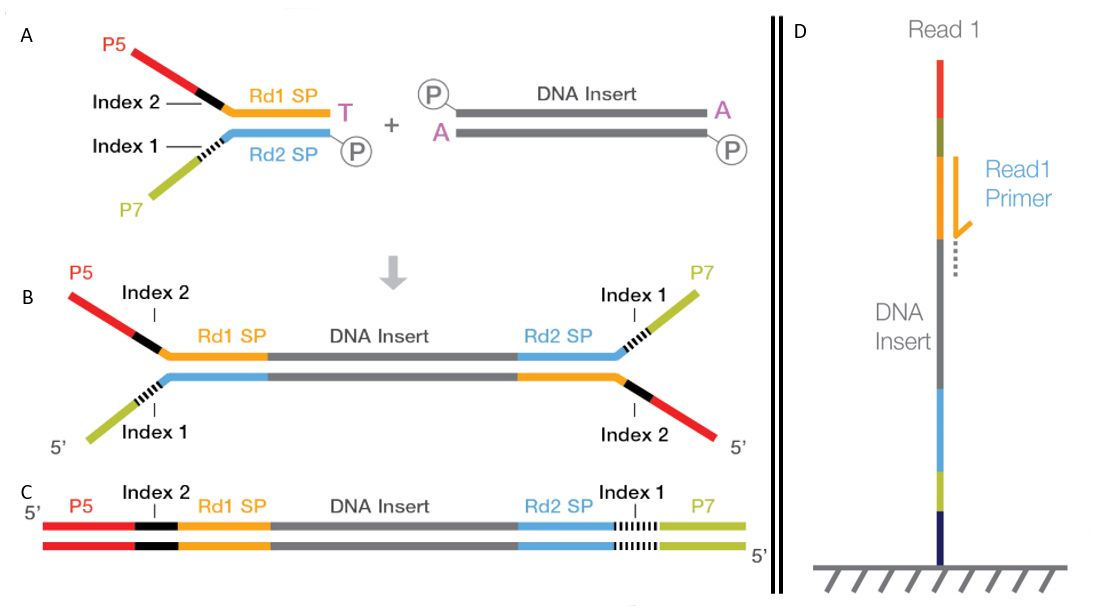
\includegraphics[width=.9\linewidth]{Figures/intro/LibraryPreparation.png}
\caption[Library preparation for NGS]{Adapter ligation during library preparation. The adapters are added to the DNA insert during library preparation. A. The DNA insert is prepared by adding an A-tail and phosphorylation. B. The adapter complex which includes the P5/P7 flow cell binding adapter is added to the DNA insert. C. The DNA insert is ready for sequencing. D. The DNA insert binds to the flow cell for sequencing. Primers bind to the DNA insert to generate reads; Figure adapted from \href{https://sapac.support.illumina.com/bulletins/2020/12/how-short-inserts-affect-sequencing-performance.html}{"How short inserts affect sequencing performance"}~\protect\cite{Illumina2020}}\label{fig:libraryprep}
\end{figure}

Library preparation is the name of the preprocessing step, which is done before it is sequenced with the current technologies. The first step to sequence DNA is to obtain the DNA, which is done by lysing the cells of interest, which disrupts the cell membrane and therefore spills all its contents. The then spilled DNA is fragmented into smaller pieces, by either restriction enzymes or sonication, to have a size of about between 200-800bp. These steps are not necessary when preparing sequencing of ctDNA, as discussed in \autoref{intro-sec:ctDNA}, as the DNA is unbound and already digested into short fragments.
Once the DNA is ready, it is phosphoryelated and an A-tail is added, before the adapter complex is ligated. This enables the DNA to bind to the flow cell which is covered with the reverse complement of the adapter (\autoref{fig:libraryprep}). 

\subsection{Next generation sequencing}
\label{intro-sec:ngs}

\begin{figure}[htp]
\centering
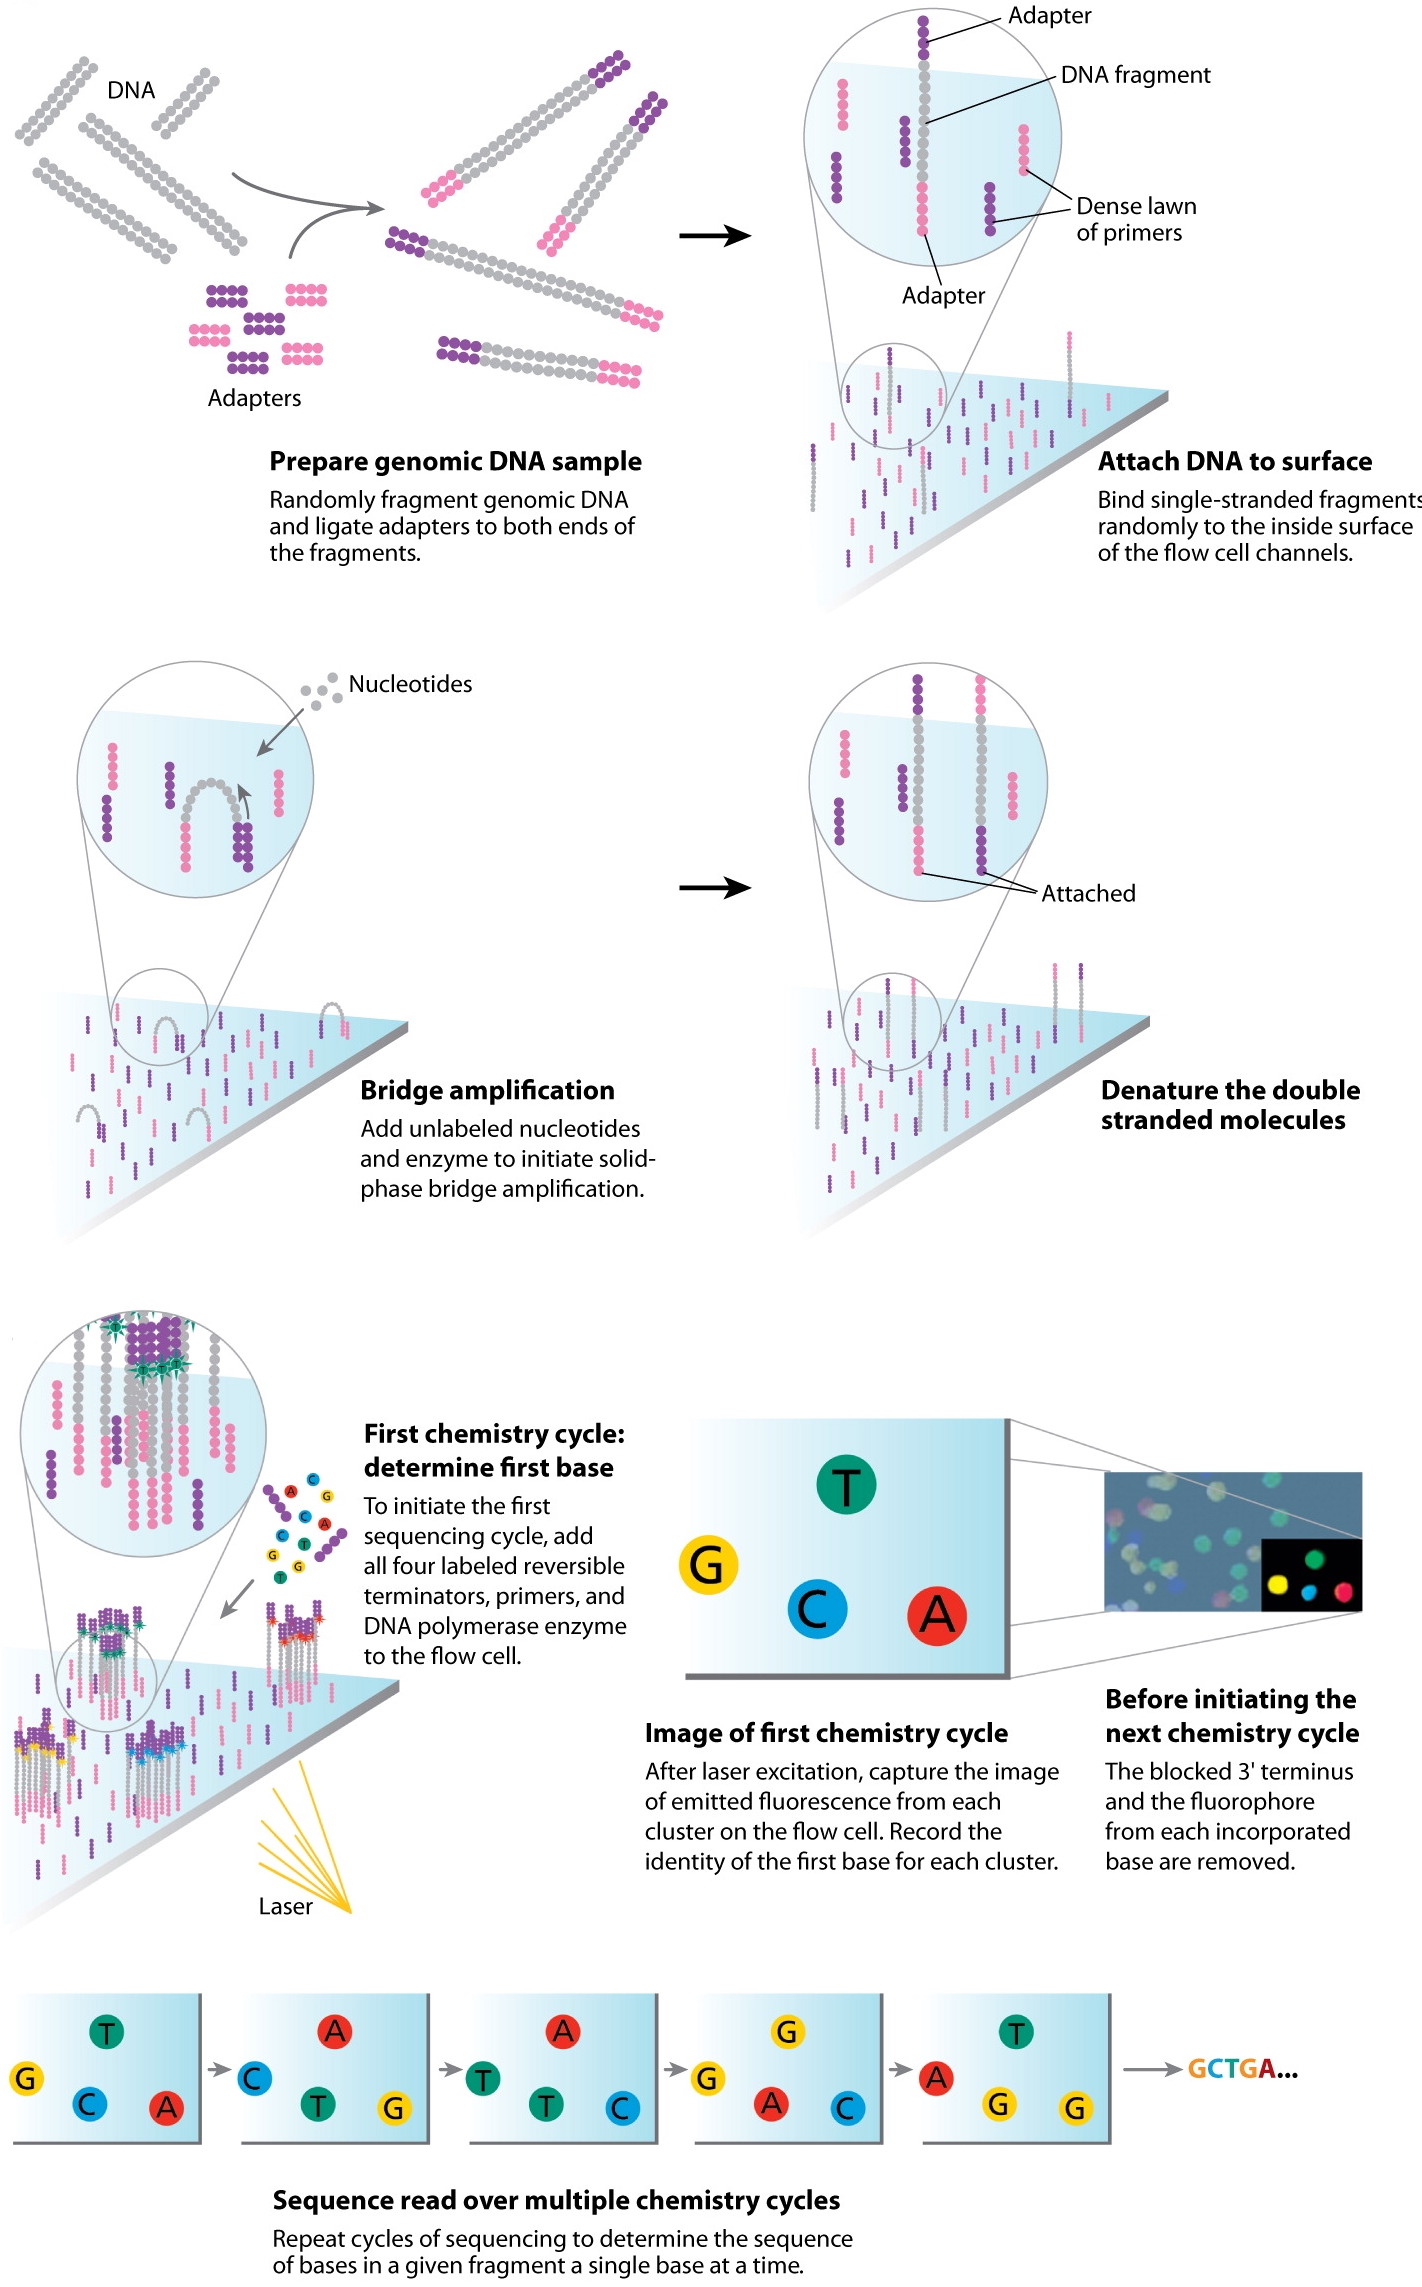
\includegraphics[width=.85\linewidth]{Figures/intro/SequencingBySynthesis.jpg}
\caption[Sequencing by synthesis (Illumina)]{The Illumina sequencing-by-synthesis approach. Cluster strands created by bridge amplification are primed and all four fluorescently labeled, 3'-OH blocked nucleotides are added to the flow cell with DNA polymerase. The cluster strands are extended by one nucleotide. Following the incorporation step, the unused nucleotides and DNA polymerase molecules are washed away, a scan buffer is added to the flow cell, and the optics system scans each lane of the flow cell by imaging units called tiles. Once imaging is completed, chemicals that effect cleavage of the fluorescent labels and the 3'-OH blocking groups are added to the flow cell, which prepares the cluster strands for another round of fluorescent nucleotide incorporation; Figure adapted from \protect\citeauthor*{Mardis2008}~\protect\cite{Mardis2008}}\label{fig:sequencingbysynthesis}
\end{figure}


Next generation sequencing (NGS) is the coined term for basically any standard high-throughput sequencing performed, which includes exome, genome, transcriptome, \linebreak protein-dna interactions (ChIP) and other epigenome studies. The term NGS is still widely used, even though it has been more than 10 years since the first NGS approach was commercially available. While in the beginning of next generation sequencing there were multiple approaches, the current lion share (80\% of sequencing data) of protocols use the Illumina short read sequencing by synthesis approach (\autoref{fig:sequencingbysynthesis}) \cite{Mardis2008,Straiton2019}, which is based on the concept of alternating integration of flourescently labelled nucleotides and imaging with a microscope (\autoref{fig:sequencingbysynthesis}) as well as multiplexing, where a DNA fragment is ligated to an index, which allows sequencing of multiple samples at once \cite{Church1984,Church1988} as it is shown in \autoref{fig:libraryprep}. This method enables highly accurate determination of the sequence of a DNA fragment and depending on the flow cell and sequencing machine allows one to sequence a whole genome in just 24h.

\subsection[Long read sequencing]{Long read sequencing - the "third" generation sequencing}
\label{intro-sec:lrs}
By now, multiple methods which broke free of the size limitations of NGS exist, which are commonly referred to as long read sequencing. Most of the current methods trade the very high accuracy of the second generation NGS methods for the capability of sequencing huge continuous strands of DNA (current record 2.3 Million bp \cite{Payne2018}) with normal library preparation ranging between 10-30 Kbp. 
These methods are expected to revolutionise our understanding of the highly repetitive elements that exist in the genome, such as the centromeres of chromosomes. Methods such as the direct molecule sequencing approach by Oxford Nanopore are even able to distinguish post transcriptional modifications on RNA \cite{Pratanwanich2021}.
However, for ctDNA, which is highly fragmented, these methods offer only limited advantages over the short read sequencing.

